\documentclass[12pt, a4paper]{amsart} 
\usepackage[utf8]{inputenc}
\usepackage[spanish]{babel}
\usepackage{anysize}
\usepackage{amsthm}
\usepackage{multicol}
\newcommand{\noun}[1]{\textsc{#1}}
\usepackage{amsmath}
\usepackage{amsfonts}
\usepackage{amssymb}
\usepackage{graphicx}
\usepackage{amscd}
\usepackage[colorlinks=true,linktocpage=true,pagebackref=true, citecolor=red,linkcolor=blue]{hyperref}
\usepackage{eurosym}
%opening

\newtheorem{teorema}{Teorema}[section]
\newtheorem{definicion}[teorema]{Definición}
\newtheorem{prop}[teorema]{Proposición}
\newtheorem{obs}[teorema]{Observación}
\newtheorem{cor}[teorema]{Corolario}
\newtheorem{ejem}[teorema]{Ejemplo}
\newtheorem{ejems}[teorema]{Ejemplos}
\newtheorem{ejer}{Ejercicio}

\newcommand{\s}{\color[rgb]{0,0,0.5}}
\newcommand{\n}{\color[rgb]{0,0,0}}


\marginsize{2cm}{2cm}{1cm}{1cm}

\begin{document}


\title{Ejercicios de programación lineal PAU - Matemáticas aplicadas a las CCSS II}
\maketitle
\date{}
\thispagestyle{empty}

\begin{ejer}\em (2021-2022)\\
La plataforma digital Plusfix va a lanzar un nuevo canal de cine y deporte y tiene que elaborar una propuesta piloto de contenidos, teniendo en cuenta que el tiempo dedicado al cine no puede ser mayor que el tiempo dedicado al deporte. La propuesta piloto debe tener una duración entre 600 y 900 minutos, debe tener al menos 200 minutos de cine y como mucho 500 minutos de deporte. Además, con la emisión de la propuesta la plataforma obtiene 15\euro\ de beneficio por cada minuto de emisión de cine y 10\euro\ de beneficio por cada minuto de emisión de deporte. Determine cuántos minutos de cine y cuántos de deporte debe tener la propuesta para obtener el máximo beneficio y obtenga el beneficio que obtiene la plataforma con dicha propuesta.
\end{ejer}

\begin{ejer}\em (2021-2022)\\
Sea $S$ la región del plano definida por
\[7y - 8x\leq 3400,\hspace*{1cm} 3x-8y\leq 2000,\hspace*{1cm} 11x+14y\geq 9500,\hspace*{1cm} x\leq 1200,\hspace*{1cm} y\leq 1000.\]
a) Represente gráficamente la región $S$ y calcule las coordenadas de sus vértices.\\
b) Obtenga el valor mínimo de la función $f(x, y) = 2x + y$ en $S,$ indicando el punto de la región en el cual se alcanza.
\end{ejer}

\begin{ejer}\em (2021-2022)\\
Un almacén de legumbres al por mayor tiene sacos de dos tipos, con capacidad para 5 kg de peso y con capacidad para 10 kg de peso. Solo tiene 180 sacos de capacidad 10 kg. Debe poner a la venta como mucho 2000 kg de alubias en sacos de ambos tipos. Por cada 3 sacos de 10 kg puede vender como mucho 2 sacos de 5 kg, y como mínimo tiene que poner a la venta 20 sacos de 5 kg y 60 de 10 kg. Por cada saco de 10 kg obtiene un beneficio de 5\euro\ y por cada saco de 5 kg obtiene un beneficio de 2\euro. Determine cuántos sacos de cada tipo debe vender para obtener el máximo beneficio y calcule el beneficio que se obtiene.
\end{ejer}

\begin{ejer}\em (2021-2022)\\
El dueño de una empresa que organiza fiestas infantiles quiere hacer chocolate con leche y dispone para la mezcla de 30 litros de leche y 20 litros de chocolate líquido. Por cada litro de chocolate
debe echar como máximo 3 litros de leche, y por cada litro de leche debe echar como máximo 1,6 litros de chocolate. Además, solo dispone de botellas para envasar 45 litros de chocolate con leche. Por cada litro de leche de la mezcla puede obtener un beneficio de 1\euro y por cada litro de chocolate un beneficio de 2\euro. Determine cuántos litros de leche y de chocolate líquido debe mezclar para obtener el máximo beneficio y calcule el beneficio que se obtiene.
\end{ejer}

\begin{ejer}\em (2020-2021)\\
Una empresa tecnológica se plantea la producción y lanzamiento de dos nuevos cables de fibra óptica, el modelo A2020 y el modelo B2020. El coste de producir un metro del modelo A2020 es igual a 2 euros, mientras que el coste de producir un metro del modelo B2020 es igual a 0, 5 euros. Para realizar el lanzamiento comercial se necesitan al menos 6000 metros de cable, aunque del modelo B2020 no podrán fabricarse más de 5000 metros y debido al coste de producción no es posible fabricar más de 8000 metros entre los dos modelos. Además se desea fabricar una cantidad de metros del modelo B2020 mayor o igual a la de metros del modelo A2020.\\
a) Represente la región factible y calcule las coordenadas de sus vértices.\\
b) Determine el número de metros que deben producirse de cada uno de los modelos para minimizar el coste.
\end{ejer}

\newpage


\s
Llamamos $x$ a los metros de cable que deben producirse del modelo A2020 e $y$ a los metros de cable que deben producirse del modelo B2020.\\

La región factible viene dada por las restricciones:

\[6000\leqslant x+y \leqslant 8000\]
\[y\leqslant 5000\]
\[y\geqslant x\]
\[x\geqslant 0, y\geqslant 0\]

Representamos la región factible:
\begin{center}
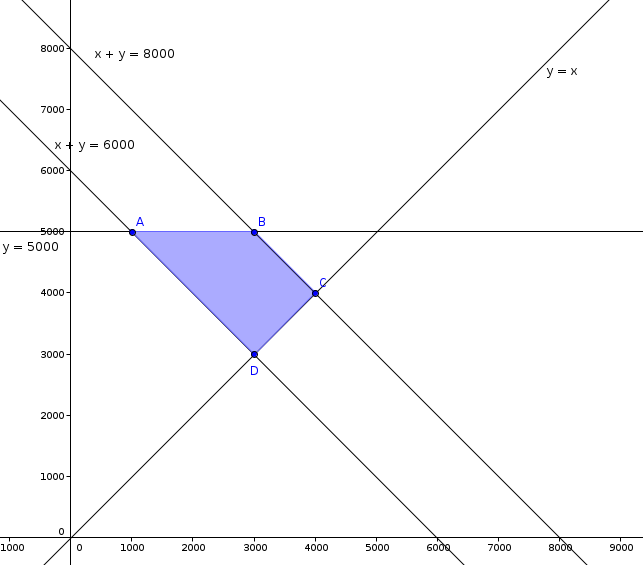
\includegraphics[scale=0.5]{2021Cable.png}
\end{center}

Los vértices de la región factible son los puntos $A=(1000,5000), B=(3000,5000), C=(4000,4000)$ y $D=(3000,3000).$


b) La función objetivo del problema es \[Min f(x,y)=2x+0,5y\] 

La solución óptima se encuentra en uno de los vértices:

$A=(1000,5000) \rightarrow f(A)=4500$ Mínimo\\

$B=(3000,5000) \rightarrow f(B)=8500$\\

$C=(4000,4000) \rightarrow f(C)=10000$\\

$D=(3000,3000) \rightarrow f(D)=7500$\\

Para minimizar el coste se deben producir 1000 metros de cable A2020 y 5000 metros de cable B2020.
\n

\begin{ejer}\em (2020-2021)\\
Un almacén de frutos secos tiene un saco de 50 kg de almendras y otro de 25 kg de avellanas. Quiere mezclarlos para preparar bolsas mixtas para su venta. La cantidad de almendras de la mezcla ha de ser como mínimo 1,5 veces la cantidad de avellanas. Además, para que le sea rentable la preparación, deberá vender al menos 60 kg entre ambos tipos de frutos secos. Por otra parte, no puede vender más de 70 kg entre ambos. Represente la región factible. Calcule la cantidad de cada fruto seco que ha de contener la mezcla para obtener el máximo beneficio si un kg de almendras le deja un beneficio de 1 \euro\ y un kg de avellanas de 2 \euro\ , y obtenga el beneficio que se obtiene con la venta de esta mezcla.
\end{ejer}
 \s 
 
Llamamos $x$ a los kg de almendras e $y$ a los kg de avellanas que contendrá la mezcla.

Se trata de Max $f(x,y)=x+2y$

Sujeto a las restricciones:
\[x\leqslant 50\]
\[y\leqslant 25\]
\[x\geqslant 1,5y\]
\[60\leqslant x+y \leqslant 70\]
\[x\geqslant 0, y\geqslant 0\]


Representamos la región factible:
\begin{center}
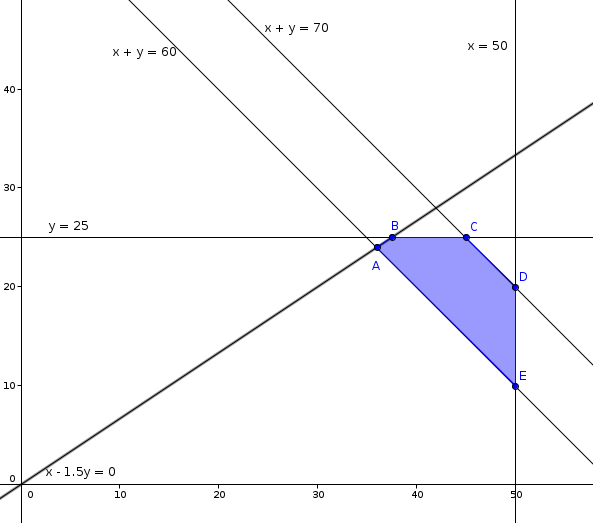
\includegraphics[scale=0.3]{2021Almendras.png}
\end{center}


Los vértices de la región factible son los puntos $A=(36,24), B=(35,25), C=(45,25), D=(50,20)$ y $E=(50,10).$

La solución óptima se encuentra en uno de los vértices, por lo que evaluamos en ellos la función objetivo:

$A=(36,24) \rightarrow f(A)=84$\\

$B=(35,25) \rightarrow f(B)=85$\\

$C=(45,25) \rightarrow f(C)=95$ Máximo\\

$D=(50,20) \rightarrow f(D)=90$\\

$E=(50,10) \rightarrow f(E)=70$\\

El máximo beneficio se obtendrá con una mezcla de 45 kg de almendras y 25 kg de avellanas.

\n

\begin{ejer}\em (2019-2020)\\
Un vivero elabora dos tipos de sustratos. Para elaborar 1 $m^3$ del tipo A necesita 60 kg de tierra vegetal y 30 horas de trabajo. Para elaborar 1 $m^3$ del tipo B necesita 50 kg de tierra vegetal y 50 horas de trabajo. El vivero
dispone como máximo de 21000 kg de tierra vegetal y 15000 horas de trabajo. Además, la cantidad de metros cúbicos que elabora de tipo A debe ser como mucho cinco veces la cantidad de tipo B. Por la venta de cada metro cúbico de tipo A obtiene un beneficio de 50 \euro\ y 60 \euro\ por cada metro cúbico de tipo B.\\
a) Represente la región del plano determinada por las restricciones anteriores y determine las coordenadas de sus vértices.\\
b) Determine cuántos metros cúbicos de cada tipo deben elaborarse para, respetando las restricciones anteriores, maximizar el beneficio. Obtenga el valor del beneficio máximo.
\end{ejer}
\s
Llamamos $x$ a la cantidad de sustrato de tipo A, en metros cúbicos, e $y$ a la cantidad de sustrato de tipo B, en metros cúbicos, que debe producirse.

a) La región factible está determinada por las restricciones:

\[Max f(x,y)=50x+60y\]
\[60x+50y\leqslant 21000\]
\[30x+50y\leqslant 15000\]
\[x\leqslant 5y\]
\[x\geqslant 0, y\geqslant 0\]


Representamos la región factible:
\begin{center}
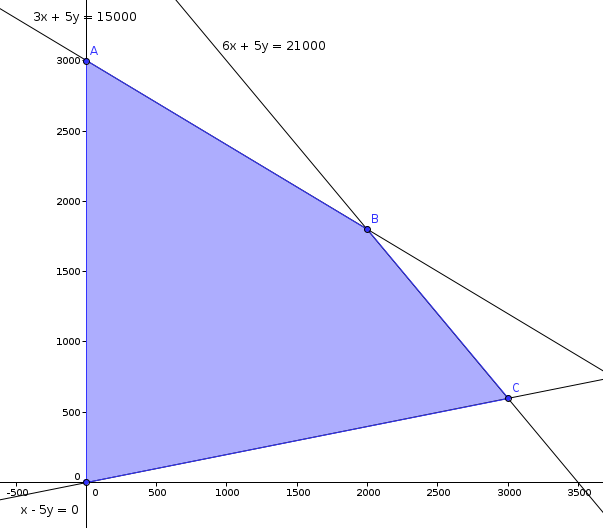
\includegraphics[scale=0.5]{2020Sustratos.png}
\end{center}



Los vértices de la región factible son los puntos $A=(0,3000), B=(2000,1800), C=(3000,600)$ y el origen de coordenadas $O=(0,0).$


b) Se quiere maximizar la función objetivo $f(x,y)=50x+60y.$ La solución óptima se encontrará en uno de los vértices, por lo que evaluamos la función objetivo en ellos:

$A=(0,3000) \rightarrow f(A)=180000$\\

$B=(2000, 1800) \rightarrow f(B)=208000$ Máximo\\

$C=(3000, 600) \rightarrow f(C)=186000$\\

$O=(0,0) \rightarrow f(O)=0$\\

Para obtener el máximo beneficio, 208.000 euros, se deben elaborar 2000 kg de sustrato de tipo A y 1800 kg de sustrato de tipo B.

\n

\begin{ejer}\em (2019-2020)\\
La región del plano S está definida por las siguientes expresiones:
\[
x\geq 3, 0\leq y\leq 15, y-5+\frac{x}{2}\geq 0, y-x\leq 10, y+20\geq 2x
\]
a) Determine las coordenadas de sus vértices y represente en el plano la región $S.$\\
b) Obtenga el valor máximo y el valor mínimo de la función $f (x, y) = x + y$ en esta región, indicando los puntos en los cuales se alcanzan estos valores.
\end{ejer}
\s

a) Representamos la región S:

\begin{center}
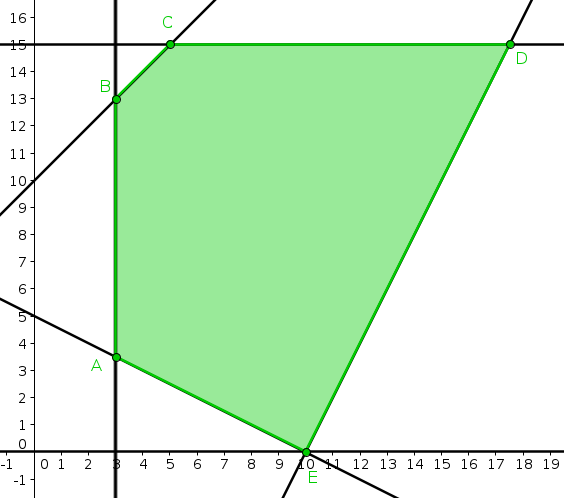
\includegraphics[scale=0.4]{2020RegionS.png}
\end{center}



Las coordenadas de sus vértices son: $A(3,\frac{7}{2}), B(3,13), C(5,15), D(\frac{35}{2}, 15)$ y $E(10,0).$

b) Evaluamos la función objetivo en los vértices
 
$A=(3;3,5) \rightarrow f(A)=6,5$ Mínimo\\

$B=(3,13) \rightarrow f(B)=16$\\

$C=(5,15) \rightarrow f(C)=20$\\

$D=(17,5; 15) \rightarrow f(D)=32,5$ Máximo\\

$E=(10,0) \rightarrow f(E)=10$\\

El valor mínimo de $f$ es 6,5 y se alcanza en el vértice $A(3;3,5),$ mientras que el valor máximo es 32,5 y se alcanza en el vértice $D(17,5; 15).$

\n

\begin{ejer}\em (2018-2019)\\
Un alcalde quiere instalar un estanque rectangular en un parque de la ciudad con las siguientes características. El estanque deberá tener al menos 2 metros de ancho y al menos 5 metros de largo. Además su largo debe ser al menos 2 veces su ancho pero no más de tres veces su ancho. Cada metro del ancho del estanque cuesta 1000 euros y cada metro de largo 500 euros. Y se cuenta con un presupuesto de 9000 euros.\\
a) Determínese la región del plano delimitada por las restricciones anteriores sobre las dimensiones del estanque.\\
b) Si se desea que el estanque respetando esas características tenga el mayor ancho posible, determínense el largo del estanque y su coste.
\end{ejer}
\s
Llamamos $x$ al ancho, en metros, del estanque, e $y$ al largo, también en metros.

a) 
Representamos la región factible:
\begin{center}
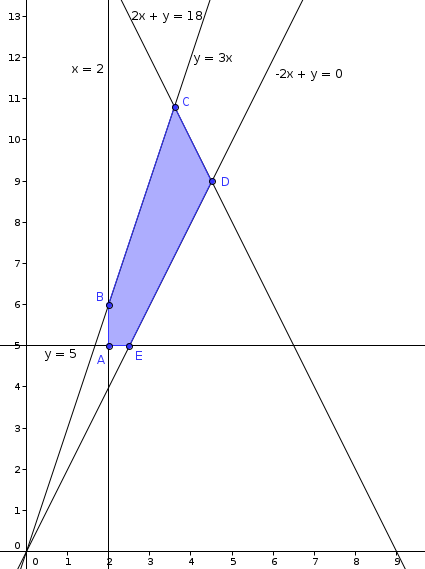
\includegraphics[scale=0.4]{2019Estanque.png}
\end{center}


La región factible está determinada por las restricciones:
\[x\geqslant 2\]
\[y\geqslant 5\]
\[2x\leqslant y \leqslant 3x\]
\[1000x+500y\leqslant 9000\]
\[x\geqslant 0, y\geqslant 0\]


Los vértices de la región factible son los puntos $A=(2,5), B=(2,6), C=(3,6; 10,8), D=(4,5; 9)$ y $E=(2,5; 5).$\\

b) Se desea maximizar el ancho, es decir, Max $f(x)=x,$ respetando las restricciones. La solución óptima se encuentra en un vértice de la región factible:

$A=(2,5) \rightarrow f(A)=2$\\

$B=(2,6) \rightarrow f(B)=2$\\

$C=(3,6; 10,8) \rightarrow f(C)=3,6$\\

$D=(4,5; 9) \rightarrow f(D)=4,5$ Máximo. Coste: $1000\cdot 4,5+500\cdot 9=9000$\\

$E=(2,5; 5) \rightarrow f(E)=2,5$\\

El estanque de máximo ancho tiene dimensiones 4,5 metros de ancho y 9 m de largo. Su coste será de 9000 euros.

\n

\begin{ejer}\em (2018-2019)\\
Una voluntaria quiere preparar helado artesano y horchata de auténtica chufa para un rastrillo solidario. La elaboración de cada litro de helado lleva 1 hora de trabajo y la elaboración de un litro de horchata 2 horas. Como la horchata no necesita leche, sabe que puede preparar hasta 15 litros de helado con la leche que tiene. Para que haya suficiente para todos los asistentes, tiene que preparar al menos 10 litros entre helado y horchata, en un máximo de 20 horas.\\
a) Represéntese la región del plano determinada por las restricciones anteriores.\\
b) Si el beneficio por litro es de 25 euros para el helado y 12 euros para la horchata, obténgase la cantidad de cada producto que se deberá preparar para maximizar el beneficio y calcúlese el beneficio máximo que podría obtenerse.
\end{ejer}
\s

Llamamos $x$ a la cantidad de helado e $y$ a la cantidad de horchata que prepara la voluntaria, ambos en litros.

a) Representamos la región factible:
\begin{center}
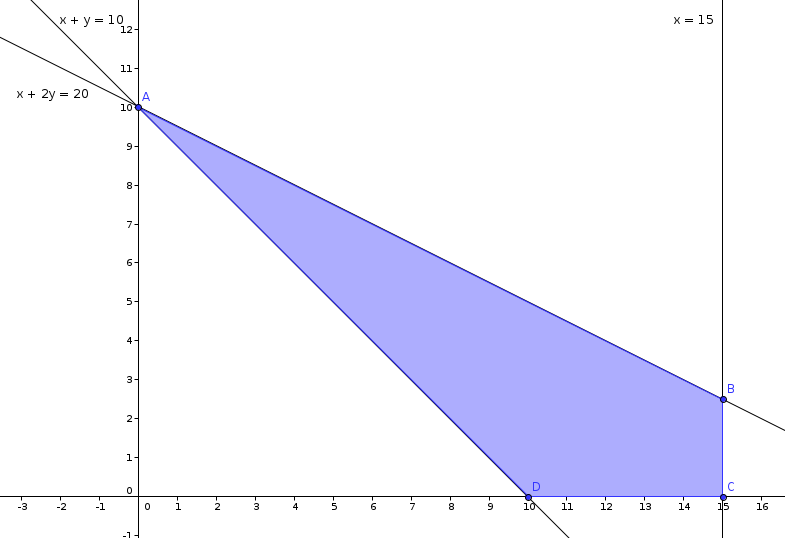
\includegraphics[scale=0.4]{2019Helado.png}
\end{center}

La región factible está determinada por las restricciones:

\[x+2y\leqslant 20\]
\[x\leqslant 15\]
\[x+y \geqslant 10\]
\[x\geqslant 0, y\geqslant 0\]


b) Se quiere maximizar la función objetivo $f(x,y)=25x+12y.$ El máximo se encontrará en uno de los vértices de la región factible $A,B,C$ o $D$:\\

$A=(0,10) \rightarrow f(A)=120$\\

$B=(15,2,5) \rightarrow f(B)=405$ Máximo\\

$C=(15,0) \rightarrow f(C)=375$\\

$D=(10,0) \rightarrow f(D)=250$\\

La voluntaria deberá preparar 15 litros de helado y 2,5 litros de horchata para alcanzar un beneficio máximo de 405 euros.



\n

\newpage

\begin{ejer}\em (2017-2018)\\
Considérese la región del plano $S$ definida por

\[
S=\{(x,y)\in \mathbb{R}^2: x+2y\geq 4; x+2y\leq 12; x\leq 4; -x+2y\leq 12\}
\]
a) Represéntese gráficamente la región $S$ y calcúlense las coordenadas de sus vértices.\\
b) Determínense los puntos en los que la función $f(x,y)= 3x - y$ alcanza sus valores máximo y mínimo en $S,$ indicando el valor de $f$ en dichos puntos.

\end{ejer}
\s

a) Representamos la región S:

\begin{center}
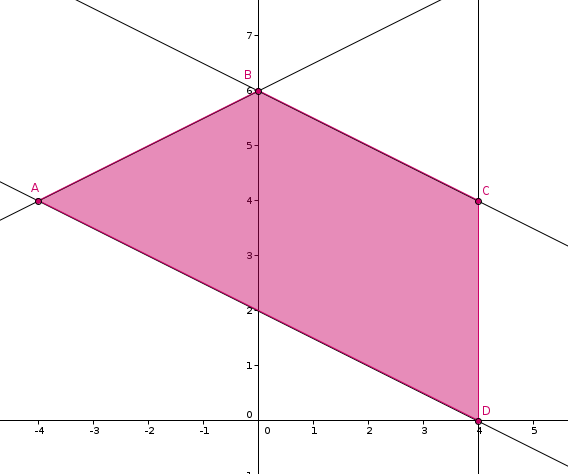
\includegraphics[scale=0.4]{2018RegionS.png}
\end{center}



Las coordenadas de sus vértices son: $A(-4,4), B(0,6), C(4,4)$ y $D(4,0).$\\

b) Evaluamos la función objetivo en los vértices
 
$A=(-4,4) \rightarrow f(A)=-16$ Mínimo\\

$B=(0,6) \rightarrow f(B)=-6$\\

$C=(4,4) \rightarrow f(C)=8$\\

$D=(4,0) \rightarrow f(D)=12$ Máximo\\

El valor mínimo de $f$ es -16 y se alcanza en el vértice $A(-4,4),$ mientras que el valor máximo es 12 y se alcanza en el vértice $D(4,0).$

\n


\begin{ejer}\em (2017-2018)\\
Sea $S$ la región del plano definida por:
\[
x+y\leq 50 ; 2x+y\leq 80 ; x\geq 0 ; y\geq 0.
\]
a) Represéntese la región $S$ y calcúlense las coordenadas de sus vértices.
b) Obténgase el valor máximo de la función $f (x, y ) = 5x + 4y$ en la región $S$, indicando el punto en el cual se alcanza dicho valor máximo.
\end{ejer}
\s


a) Las coordenadas de sus vértices son: $A(0,0), B(0,50), C(30,20), D(40,0).$\\
Representamos la región S:

\begin{center}
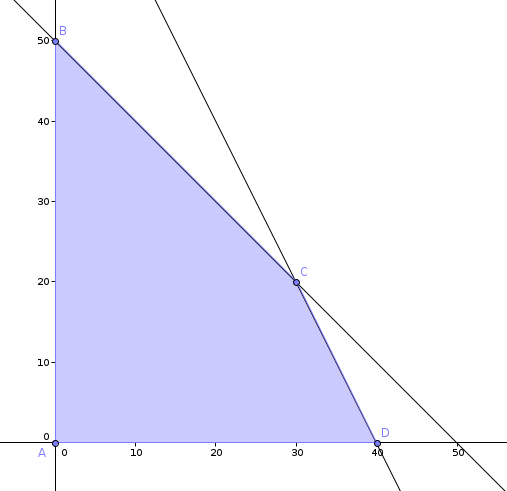
\includegraphics[scale=0.4]{2018Region.png}
\end{center}


b) Evaluamos la función objetivo en los vértices
 
$A=(0,0) \rightarrow f(A)=0$ Mínimo\\

$B=(0,50) \rightarrow f(B)=200$\\

$C=(30,20) \rightarrow f(C)=230$ Máximo\\

$D=(40,0) \rightarrow f(D)=200$\\

El valor mínimo de $f$ es 0 y se alcanza en el origen de coordenadas, mientras que el valor máximo es 230 y se alcanza en el vértice $C(40,0).$

\n

\begin{ejer}\em (2016-2017)\\
Se considera la región del plano S definida por:\\
\[
1\leq x\leq 5 ; 2\leq y \leq 6 ; x-y\geq -4 ; 3x-y\leq 10.
\]
a) Represéntese gráficamente la región $S$ y calcúlense las coordenadas de sus vértices.\\
b) Calcúlense los valores máximo y mínimo de la función $f (x, y) = - 200x + 600y$ en la región $S$ y obténganse los puntos de $S$ donde se alcanzan dichos valores.
\end{ejer}
\s

a) Representamos la región S:

\begin{center}
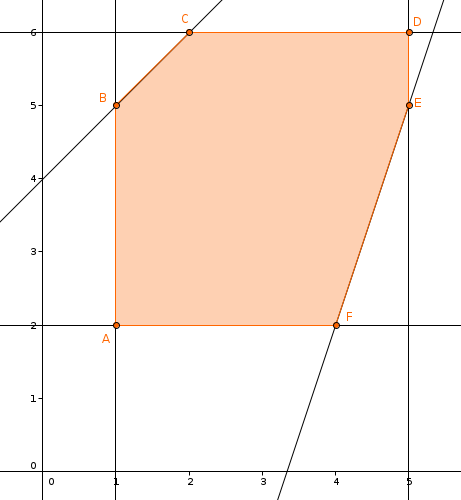
\includegraphics[scale=0.4]{2017RegionS.png}
\end{center}



Las coordenadas de sus vértices son: $A(1,2), B(1,5), C(2,6), D(5,6), E(5,5)$ y $F(4,2).$\\

\newpage

b) Evaluamos la función objetivo en los vértices
 
$A=(1,2) \rightarrow f(A)=1000$ Mínimo\\

$B=(1,5) \rightarrow f(B)=2800$\\

$C=(2,6) \rightarrow f(C)=3200$ Máximo\\

$D=(5,6) \rightarrow f(D)=2600$\\

$E=(5,5) \rightarrow f(D)=2000$\\

$F=(4,2) \rightarrow f(D)=2000$\\

El valor mínimo de $f$ en la región es 1000 y se alcanza en el vértice $A(1,2),$ mientras que el valor máximo es 3200 y se alcanza en el vértice $C(2,6).$

\n

\begin{ejer}\em (2016-2017)\\
Considérese la región del plano $S$ definida por

\[
S=\{(x,y)\in \mathbb{R}^2: x+6y\geq 6; 5x-2y\geq -2; x+3y\leq 20; 2x-y\leq 12\}
\]
a) Represéntese gráficamente la región $S$ y calcúlense las coordenadas de sus vértices.\\
b) Determínense los puntos en los que la función $f (x, y) = 4x - 3y$ alcanza sus valores máximo y mínimo en $S,$ indicando el valor de $f (x, y)$ en dichos puntos.
\end{ejer}
\s


a) Representamos la región S:

\begin{center}
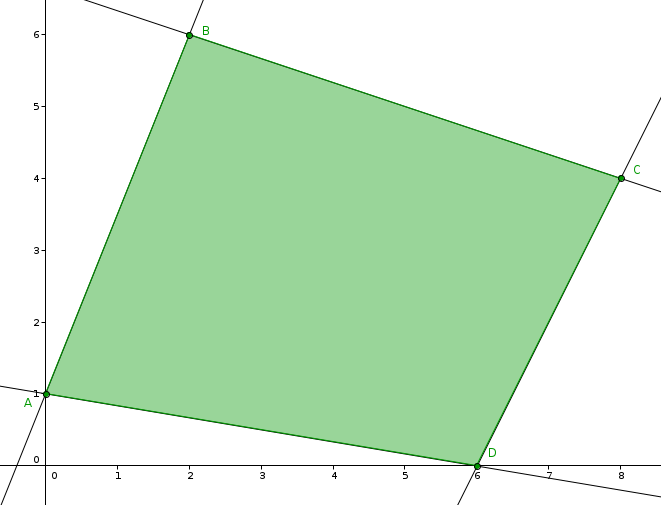
\includegraphics[scale=0.4]{2017Region.png}
\end{center}



Las coordenadas de sus vértices son: $A(0,1), B(2,6), C(8,4)$ y $D(6,0).$\\

b) Evaluamos la función objetivo en los vértices
 
$A=(0,1) \rightarrow f(A)=-3$ Mínimo\\

$B=(2,6) \rightarrow f(B)=-10$\\

$C=(8,4) \rightarrow f(C)=20$\\

$D=(6,0) \rightarrow f(D)=24$ Máximo\\

El valor mínimo de $f$ es -3 y se alcanza en el vértice $A(0,1),$ mientras que el valor máximo es 24 y se alcanza en el vértice $D(6,0).$


\n

\begin{ejer}\em (2015-2016)\\
Sea $S$ la región del plano definida por:

\[2x-y\geq 1; 2x-3y\leq 6; x+2y \geq 3; x+y\leq 8; y\leq 3.\]
\vspace*{5mm}

a) Represéntese la región $S$ y calcúlense las coordenadas de sus vértices.\\
b) Obténganse los valores máximo y mínimo de la función $f (x, y ) = 2x + y$ en la región $S$ indicando los puntos de $S$ en los cuales se alcanzan dichos valores máximo y mínimo.
\end{ejer}
\s

a) Representamos la región S:

\begin{center}
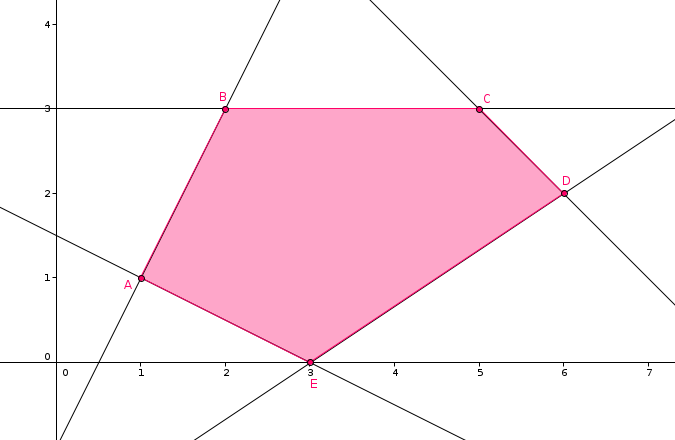
\includegraphics[scale=0.4]{2016RegionS.png}
\end{center}



Las coordenadas de sus vértices son: $A(1,1), B(2,3), C(5,3), D(6,2)$ y $E(3,0).$\\

b) Evaluamos la función objetivo en los vértices
 
$A=(1,1) \rightarrow f(A)=3$ Mínimo\\

$B=(2,3) \rightarrow f(B)=7$\\

$C=(5,3) \rightarrow f(C)=13$\\

$D=(6,2) \rightarrow f(D)=14$ Máximo\\

$E=(3,0) \rightarrow f(D)=6$\\


El valor mínimo de $f$ en la región es 3 y se alcanza en el vértice $A(1,1),$ mientras que el valor máximo es 14 y se alcanza en el vértice $D(6,2).$




\n
\begin{ejer}\em (2015-2016)\\
Sea $S$ la región del plano definida por:

\[y+x\leq 5; y-x\leq 3; \frac{1}{2}x-y\leq -2.\]
\vspace*{5mm}

a) Represéntese la región $S$ y calcúlense las coordenadas de sus vértices.\\
b) Obténganse los valores máximo y mínimo de la función $f (x, y ) = 2x + y$ en la región $S$ indicando los puntos de $S$ en los cuales se alcanzan dichos valores máximo y mínimo.
\end{ejer}
\s

a) 
Las coordenadas de sus vértices son: $A(-2,1), B(1,4)$ y $C(2,3).$\\
Representamos la región S:

\begin{center}
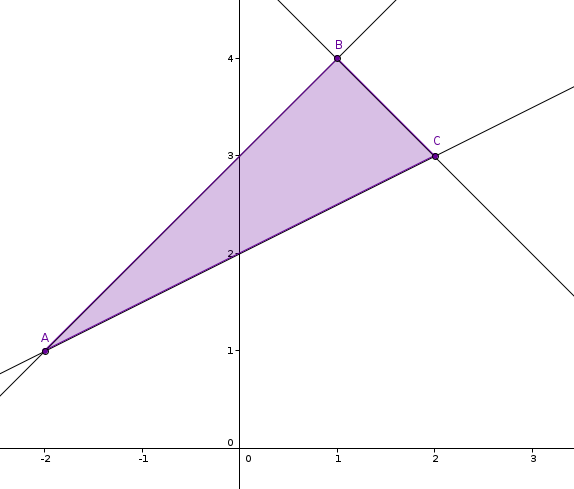
\includegraphics[scale=0.4]{2016Region.png}
\end{center}




b) Evaluamos la función objetivo en los vértices
 
$A=(-2,1) \rightarrow f(A)=-3$ Mínimo\\

$B=(1,4) \rightarrow f(B)=6$\\

$C=(2,3) \rightarrow f(C)=7$\\


El valor mínimo de $f$ en la región es -3 y se alcanza en el vértice $A(-2,1),$ mientras que el valor máximo es 7 y se alcanza en el vértice $C(2,3).$




\n

\begin{ejer}\em (2014-2015)\\
Una fábrica de piensos para animales produce diariamente como mucho seis toneladas de pienso del tipo A y como máximo cuatro toneladas de pienso del tipo B. Además, la producción diaria de pienso del tipo B no puede superar el doble de la del tipo A y, por último, el doble de la fabricación de pienso del tipo A sumada con la del tipo B debe ser como poco cuatro toneladas diarias. Teniendo en cuenta que el coste de fabricación de una tonelada de pienso del tipo A es de 1000 euros y el de una tonelada del tipo B de 2000 euros, ¿cuál es la producción diaria para que la fábrica cumpla con sus obligaciones con un coste mínimo? Calcúlese dicho coste diario mínimo.
\end{ejer}
\s
Llamamos $x$ a las toneladas de pienso de tipo A e $y$ a las toneladas de pienso de tipo B que se deben producir.

El problema de programación lineal queda definido

\[Min f(x+y)=1000x+2000y\]

\[x\leqslant 6\]
\[y\leqslant 4\]
\[y\leqslant 2x\]
\[2x+y\geqslant 4\]
\[x\geqslant 0, y\geqslant 0\]

\vspace*{1cm}

Los vértices de la región factible son los puntos $A(1,2), B(2,4), C(6,4), D(6,0)$ y $E(2,0).$

\newpage

La región factible queda representada:

\begin{center}
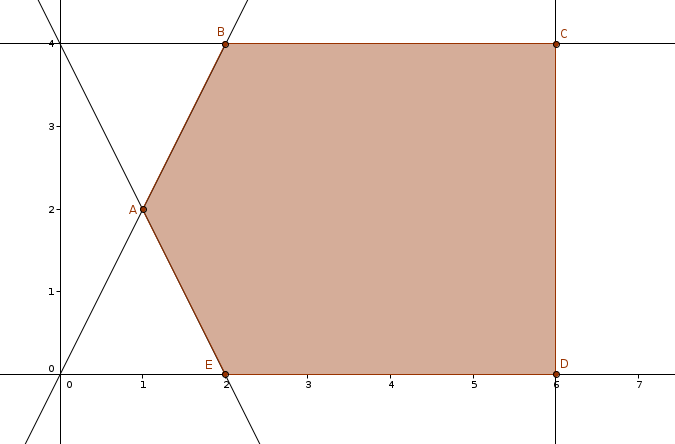
\includegraphics[scale=0.4]{2015Pienso.png}
\end{center}



La solución óptima se encuentra en uno de los vértices, por lo que evaluamos en ellos la función objetivo:

 
$A=(1,2) \rightarrow f(A)=5000$ \\

$B=(2,4) \rightarrow f(B)=10000$\\

$C=(6,4) \rightarrow f(C)=14000$\\

$D=(6,0) \rightarrow f(D)=6000$\\

$E=(2,0) \rightarrow f(D)=2000$ Mínimo\\

La fábrica de piensos cumple las obligaciones con un coste mínimo de 2000 euros si fabrica únicamente 2 toneladas de pienso de tipo A.

\n



\begin{ejer}\em (2014-2015)\\
Un distribuidor de aceite acude a una almazara a comprar dos tipos de aceite, A y B. La cantidad máxima que puede comprar es de 12.000 litros en total. El aceite de tipo A cuesta 3 euros/litro y el de tipo B cuesta 2 euros/litro. Necesita adquirir al menos 2.000 litros de cada tipo de aceite. Por otra parte, el coste total por compra de aceite no debe ser superior a 30.000 euros. El beneficio que se conseguirá con la venta del aceite será de un $25\%$ sobre el precio que ha pagado por el aceite de tipo A y de un $30\%$ sobre el precio que ha pagado por el aceite de tipo B. ¿Cuántos libros de cada tipo de aceite se deberían adquirir para maximizar el beneficio? Obténgase el valor del beneficio máximo.
\end{ejer}
\s

Llamamos $x$ a la cantidad de aceite de tipo A, en miles de litros, e $y$ a la cantidad de aceite de tipo B, también en miles de litros, que adquiere el distribuidor.

El problema de programación lineal queda definido
\[Max f(x,y)= 1250\cdot 3x+1300\cdot 2y=3750x+2600y\]
\[x+y\leqslant 12\]
\[3x+2y\leqslant 30\]
\[x\geqslant 2, y\geqslant 2\]

La región factible queda representada:

\begin{center}
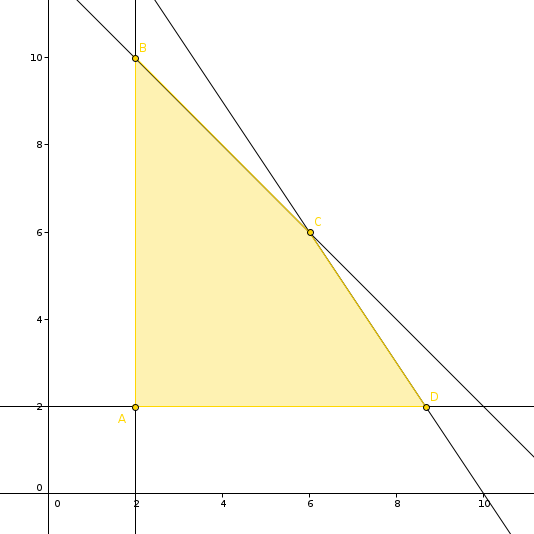
\includegraphics[scale=0.4]{2015Aceite.png}
\end{center}


Los vértices de la región factible son los puntos $A(2,2), B(2,10), C(6,6)$ y $D(26/3,2)$\\


La solución óptima se encuentra en uno de los vértices, por lo que evaluamos en ellos la función objetivo:

 
$A=(2,2) \rightarrow f(A)=12700$ \\

$B=(2,10) \rightarrow f(B)=33500$\\

$C=(6,6) \rightarrow f(C)=38100$ Máximo\\

$D=(26/3,2) \rightarrow f(D)=37700$\\

Para obtener un beneficio máximo de 38100 euros el distribuidor debe comprar 2000 litros de aceite a la almazara A y 10000 litros a la almazara B.

\n


\begin{ejer}\em (2013-2014)\\
Se consideran la función $f(x,y)=5x-2y$ y la región del plano $S$ definida por las restricciones:
\[x-2y\leq 0,\hspace*{0.5cm} x+y\leq 6,\hspace*{0.5cm} x\geq 0,\hspace*{0.5cm} y\leq 3.\]
a) Represéntese la región $S.$\\
b) Calcúlense las coordenadas de los vértices de la región $S$ y obténgase los valores de la función $f$ en $S$ indicando los puntos donde se alcanzan.
\end{ejer}
\s

\n

\begin{ejer}\em  (2013-2014)\\
Sea $S$ la región del plano definida por
$y\geq 2x-4; y\leq x-1; 2y\geq x; x\geq 0; y\geq 0.$\\
a) Represéntese la región $S$ y calcúlense las coordenadas de sus vértices.\\
b)Obténgase los valores máximo y mínimo de la función $f(x,y)=x-3y$ en $S$ indicando los puntos de $S$ en los cuales se alcanzan dichos valores máximo y mínimo.
\end{ejer}
\s

\n

\begin{ejer}\em (2012-2013)\\
Se desea maximizar la función $f(x,y)=64,8x+76,5y$ sujete a las siguientes restricciones:
\[6x+5y\leq 700,\hspace*{0.5cm} 2x+3y\leq 300,\hspace*{0.5cm} x\geq 0,\hspace*{0.5cm} y\geq 0\]
a) Represéntese gráficamente la región de soluciones factibles y calcúlense las coordenadas de sus vértices.\\
b) Determínese el valor máximo de $f$ sobre la región, indicado el punto donde se alcanza dicho máximo.
\end{ejer}
\s

\n

\begin{ejer}\em (2012-2013)\\
Sea $C$ la región del plano delimitada por el sistema de inecuaciones
\begin{equation*}
\left \{ \begin{matrix} x+3y\geq 3
\\ 2x-y\leq 4
\\ 2x+y\leq 24
\\ x\geq 0, y\geq 0 \end{matrix}\right. 
\end{equation*}
a) Represéntese la región $C$ y calcúlense las coordenadas de sus vértices.\\
b) Determínese el punto de $C$ donde la función $f(x,y)=3x+y$ alcanza su valor máximo. Calcúlese dicho valor.
\end{ejer}
\s

\n


\begin{ejer}\em (2011-2012)\\
Un pintor dispone de dos tipos de pintura para realizar su trabajo. El primer tipo de pintura tiene un rendimiento de 3 $m^2$ por litro, con un coste de 1\euro\ por litro. 
El segundo tipo de pintura tiene un rendimiento de 4 $m^2$ por litro, con un coste de 1,2\euro\ por litro. Con ambos tipos de pintura se puede pintar a un ritmo de 1 litro cada 10 minutos. El pintor dispone de un presupuesto de 480\euro\ y no puede pintar durante más de 75 horas. Además, debe utilizar al menos 120 litros de cada tipo de pintura.\\
Determínese la cantidad de pintura que debe utilizar de cada tipo si su objetivo es pintar la máxima superficie posible. Indíquese cuál es esa superficie máxima.
\end{ejer}
\s
Llamamos $x$ a la cantidad de pintura del primer tipo, en litros, e $y$ a la cantidad de pintura el segundo tipo, también en litros, que compra el pintor.

El problema de programación lineal queda definido
\[Max f(x,y)= 3x+4y\]
\[x+1,2y\leqslant 480\]
\[10(x+y)\leqslant 4500\]
\[x\geqslant 120, y\geqslant 120\]

%La región factible queda representada:


%Los vértices de la región factible son los puntos



%La solución óptima se encuentra en uno de los vértices, por lo que evaluamos en ellos la función objetivo:

\n

\begin{ejer}\em (2010-2011)\\
Se considera la región $S$ acotada plana definida por las cinco condiciones siguientes:
\[x+2y\leqslant 4;\hspace*{1cm} x-2y\leqslant 4;\hspace*{1cm} 2x-3y\geqslant -6;\hspace*{1cm} 2x+3y\geqslant -6;\hspace*{1cm} x\leqslant 2\]
a) Dibújese $S$ y calcúlense las coordenadas de sus vértices.\\
b) Calcúlense los valores máximo y mínimo de la función $f(x,y)=2x+y$ en la región $S$ y especifíquese los puntos de $S$ en los cuales se alcanzan dichos valores máximo y mínimo.
\end{ejer}



\begin{ejer}\em (2009-2010)\\
Se considera la función $f(x,y)=-0,4x+3,2y$\\
sujeta a las restricciones: \[\left \{ \begin{matrix}
x+y\leq 7
\\ x+4y\geq 4
\\ x+5\geq y\\
0\leq x\leq 5,\\
 y\geq 0
\end{matrix}\right.\]
a) Represéntese la región $S$ del plano determinada por el conjunto de restricciones.\\
b) Calcúlense los puntos de la región $S$ donde la función $f$ alcanza sus valores máximo y mínimo.\\
c) Calcúlense dichos valores máximo y mínimo.
\end{ejer}
\s

\n

\begin{ejer}\em  (2009-2010)\\
Un club de fútbol dispone de un máximo de 2 millones de euros para fichajes de futbolistas españoles y extranjeros. Se estima que el importe total de las camisetas vendidas por el club con el nombre de futbolistas españoles es igual al $10\%$ de la cantidad total invertida por el club en fichajes de españoles, mientras que el importe total de las camisetas vendidas con el nombre de futbolistas extranjeros es igual al $15\%$ de la cantidad total invertida por el club en fichajes de extranjeros. Los estatutos del club limitan a un máximo de 800.000 euros la inversión total en fichajes extranjeros y exigen que la cantidad total invertida en fichajes de futbolistas españoles sea como mínimo de 500.000 euros. Además, la cantidad total invertida en fichajes de españoles ha de ser mayor o igual que la invertida en fichajes extranjeros. ¿Qué cantidad debe invertir el club en cada tipo de fichajes para que el importe de las camisetas vendidas sea máximo? Calcúlese dicho importe máximo. Justifíquese.
\end{ejer}
\s
Llamamos $x$ al dinero invertido en futbolistas españoles e $y$ al dinero invertido en fichajes extranjeros, ambos en miles de euros.

El problema de programación lineal queda definido
\[Max f(x,y)= 0,1x+0,15y\]
\[x+y\leqslant 2000\]
\[y\leqslant 800\]
\[x\geqslant 500\]
\[x\geqslant y\]
\[x\geqslant 0, y\geqslant 0\]

%La región factible queda representada:


%Los vértices de la región factible son los puntos



%La solución óptima se encuentra en uno de los vértices, por lo que evaluamos en ellos la función objetivo:

\n

\begin{ejer}\em  (2009-2010)\\
Un pintor necesita pintura para pintar como mínimo una superficie de $480 m^2.$ Puede comprar la pintura a dos proveedores, A y B. El proveedor A le ofrece una pintura con un rendimiento de 6 $m^2$ por kg y un precio de 1 euro por kg. La pintura del proveedor B tiene un precio de 1,2 euros por kg y un rendimiento de 8 $m^2$ por kg. Ningún proveedor le puede proporcionar más de 75 kg de pintura y el presupuesto máximo del pintor es de 120 euros. Calcúlese la cantidad de pintura que el pintor tiene que comprar a cada proveedor para obtener el mínimo coste. Calcúlese dicho coste mínimo. 
\end{ejer}
\s

\n

\begin{ejer}\em  (2009-2010)\\
Un grupo inversor dispone de un máximo de 9 millones de euros para invertir en dos tipos de fondos de inversión, A y B. El fondo de inversión del tipo A tiene una rentabilidad del $4\%$ anual y una limitación legal de 5 millones de euros de inversión máxima. El fondo de inversión del tipo B tiene una rentabilidad del $3\%$ anual, deben invertirse al menos 2 millones de euros y no hay límite superior de inversión. El grupo inversor desea invertir en el fondo del tipo B, como máximo, el doble de lo invertido en el fondo del tipo A. ¿Qué cantidad debe invertir el grupo en cada tipo de fondo para obtener el máximo beneficio anual? Calcúlese dicho beneficio máximo.
\end{ejer}
\s

\n



\begin{ejer}\em  (2008-2009)\\
Una refinería utiliza dos tipos de petróleo, A y B, que compra a un precio de 350 euros y 400 euros por tonelada, respectivamente. Por cada tonelada de petróleo de tipo A que refina, obtiene 0,10 toneladas de gasolina y 0,35 toneladas de fuel-oil. Por cada tonelada de petróleo de tipo B que refina, obtiene 0,05 toneladas de gasolina y 0,55 toneladas de fuel-oil. Para cubrir sus necesidades necesita obtener al menos 10 toneladas de gasolina y al menos 50 toneladas de fuel-oil. Por cuestiones de capacidad, no puede comprar más de 100 toneladas de cada tipo de petróleo. ¿Cuántas toneladas de petróleo de cada tipo debe comprar la refinería para cubrir sus necesidades a mínimo coste? Determinar dicho coste mínimo.
\end{ejer}

\begin{ejer}\em  (2008-2009)\\
Una carpintería vende paneles de contrachapado de dos tipos A y B. Cada $m^2$ de panel de tipo A requiere 0,3 horas de trabajo para su fabricación y 0,2 horas para su barnizado, proporcionando su venta un beneficio de 4 euros. Cada $m^2$ de panel de tipo B requiere 0,2 horas de trabajo para su fabricación y 0,2 horas para su barnizado, proporcionando su venta un beneficio de 3 euros. Sabiendo que en una semana se trabaja un máximo de 240 horas en el taller de fabricación y de 200 horas en el taller de barnizado, calcular los $m^2$ de cada tipo de panel que debe vender semanalmente la carpintería para obtener el máximo beneficio. Calcular dicho beneficio máximo.
\end{ejer}


\begin{ejer}\em  (2007-2008)\\
Un distribuidor de aceite de oliva compra la materia prima a dos almazaras, A y B. Las almazaras A y B venden el aceite a 2000 y 3000 euros por tonelada, respectivamente. Cada almazara le vende un mínimo de 2 toneladas y un máximo de 7 y para atender a su demanda, el distribuidor debe comprar en total un mínimo de 6 toneladas. El distribuidor debe comprar como máximo a la almazara A el doble de aceite que a la almazara B. ¿Qué cantidad de aceite debe comprar el distribuidor a cada una de las almazaras para obtener el mínimo coste? Determínese dicho coste mínimo.
\end{ejer}

\begin{ejer}\em  (2007-2008)\\
Se desea invertir una cantidad de dinero menor o igual que 125000 euros, distribuidos entre acciones de tipo A y del tipo B. Las acciones del tipo A garantizan una ganancia del $10\%$ anual, siendo obligatorio invertir en ellas un mínimo de 30000 euros y un máximo de 81000 euros.Las acciones del tipo B garantizan una ganancia del $5\%$ anual, siendo obligatorio invertir en ellas un mínimo de 25000 euros. La cantidad invertida en acciones del tipo B no puede superar el triple de la cantidad invertida en acciones del tipo A. ¿Cuál debe ser la distribución de la inversión para maximizar la ganancia anual? Determínese dicha ganancia máxima.
\end{ejer}


\begin{ejer}\em  (2006-2007)\\
Una empresa de instalaciones dispone de 195 kg de cobre, 20 kg de titanio y 14 kg de aluminio. Para fabricar 100 metro de cable de tipo A se necesitan 10 kg de cobre, 2 de titanio y 1 de aluminio, mientras que para fabricar 100 metros de cable de tipo B se necesitan 15 kg de cobre, 1 de titanio y 1 de aluminio. El beneficio que se obtiene por 100 metros de cable de tipo A es de 1500 euros, y por 100 metros de cable de tipo B, 1000 euros.\\
Calcular los metros de cable de cada tipo que hay que fabricar para maximizar el beneficio de la empresa. Obtener dicho beneficio máximo.
\end{ejer}
\s

\hspace*{-4mm} a) Definimos las variables:\\
$x:$ cantidad de cable A (en cientos de metros)\\
$y:$ cantidad de cable B (en cientos de metros)

Función objetivo: Max $f(x,y)=1500x+1000y$\\

Restricciones:\\
$10x+15y\leqslant 195$\\
$2x+y\leqslant 20$\\
$x+y\leqslant 14$\\
$x\geqslant 0, y\geqslant 0$\\

Representamos la región factible:

\begin{center}
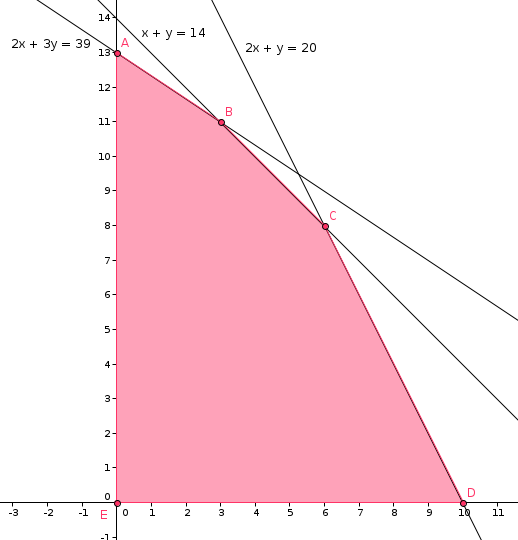
\includegraphics[scale=0.5]{2007 Cable.png}
\end{center}

b) Calculamos los vértices:

\[A=(0,13),B=(3,11), C=(6,8), D=(10,0), E=(0,0)\]

Evaluamos la función objetivo en cada vértice:

\[f(A)=1500\cdot 0+1000\cdot 13=13000; f(B)=15500; f(C)=17000 \text{ Máximo}; f(D)=15000; f(E)=0\]

\vspace*{5mm}

Se deben fabricar 600 metros de cable tipo A y 800 metros de cable tipo B para obtener el beneficio máximo de 17000 \euro.


\n

\begin{ejer}\em  (2006-2007)\\
Una aerolínea quiere optimizar el número de filas de clase preferente y de clase turista en un avión. La longitud útil del avión para instalar las filas de asientos es de 104 , necesitándose 2 m  para instalar una fila de clase preferente y 1,5   para las de clase turista. La aerolínea precisa instalar al menos 3 filas de clase preferente y que las filas de clase turista sean como mínimo el triple que las de clase preferente. Los beneficios por fila de clase turista son de 152 euros y de 206 euros para la clase preferente.\\
¿Cuántas filas de clase preferente y cuántas de clase turista se deben instalar para obtener el beneficio máximo? Indicar dicho beneficio.
\end{ejer}
\s

\hspace*{-4mm}Definimos las variables:\\
$x:$ número de filas de clase preferente\\
$y:$ número de filas de clase turista\\

\hspace*{-4mm}Función objetivo Max $f(x,y)=206x+152y$\\



\hspace*{-4mm}Restricciones:\\ 
$3x+2y\leqslant 108$\\
$x\geqslant 4$\\
$y\geqslant 3x$\\
$x\geqslant 0, y\geqslant 0$

\begin{center}
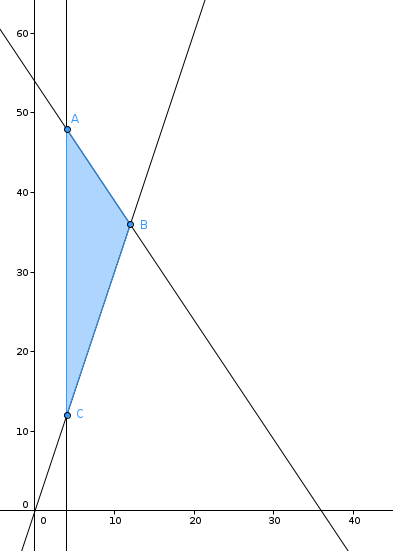
\includegraphics[scale=0.5]{2007 Aerolínea.png}
\end{center}


Vértices de la región factible: $A=(4,48), B=(12,36)$ y $C=(4,12).$

Evaluamos la función objetivo en los vértices:

\[f(A)=8120 \text{ Máximo }, f(B)=7944, f(C)=2648\]

Para obtener el máximo beneficio, que sería de 8120 euros, se deben instalar 4 filas de clase preferente y 48 filas de clase turista.

\n

\vspace*{1cm}


\end{document}

\begin{ejer}\em 

\end{ejer}
